\documentclass[conference]{IEEEtran}
\usepackage{booktabs}
\usepackage{graphicx}
\usepackage{amsmath}
\usepackage{url}
\usepackage[hidelinks]{hyperref}
\graphicspath{{../results/figures/}}
\IfFileExists{generated/numbers.tex}{\newcommand{\SIIFinalQWK}{0.827}
\newcommand{\SIIFinalAcc}{0.771}
\newcommand{\SIIFinalMF}{0.473}
\newcommand{\SIIFinalMinRec}{0.148}
\newcommand{\SIIFinalSevRec}{0.00}
\newcommand{\SIIFinalPDRRec}{0.30}
\newcommand{\SIIFinalMildRec}{0.23}
\newcommand{\SIIBestQWK}{0.827}
\newcommand{\SIIBestAcc}{0.771}
\newcommand{\SIIBestMF}{0.473}
\newcommand{\SIIBestMinRec}{0.148}
\newcommand{\SIIBestSevRec}{0.00}
\newcommand{\SIIBestPDRRec}{0.30}
\newcommand{\SIIBestMildRec}{0.23}
\newcommand{\SIIVoteQWK}{0.788}
\newcommand{\SIIVoteAcc}{0.767}
\newcommand{\SIIVoteMF}{0.412}
\newcommand{\SIIVoteMinRec}{0.000}
\newcommand{\SIIVoteSevRec}{0.00}
\newcommand{\SIIVotePDRRec}{0.00}
\newcommand{\SIIVoteMildRec}{0.29}
\newcommand{\SIIMeanQWK}{0.791}
\newcommand{\SIIMeanAcc}{0.769}
\newcommand{\SIIMeanMF}{0.416}
\newcommand{\SIIMeanMinRec}{0.000}
\newcommand{\SIIMeanSevRec}{0.00}
\newcommand{\SIIMeanPDRRec}{0.00}
\newcommand{\SIIMeanMildRec}{0.30}
\newcommand{\SIIlowFinalQWK}{0.862}
\newcommand{\SIIlowFinalAcc}{0.798}
\newcommand{\SIIlowFinalMF}{0.603}
\newcommand{\SIIlowFinalMinRec}{0.370}
\newcommand{\SIIlowFinalSevRec}{0.17}
\newcommand{\SIIlowFinalPDRRec}{0.57}
\newcommand{\SIIlowFinalMildRec}{0.46}
\newcommand{\SIIlowBestQWK}{0.887}
\newcommand{\SIIlowBestAcc}{0.815}
\newcommand{\SIIlowBestMF}{0.630}
\newcommand{\SIIlowBestMinRec}{0.428}
\newcommand{\SIIlowBestSevRec}{0.31}
\newcommand{\SIIlowBestPDRRec}{0.55}
\newcommand{\SIIlowBestMildRec}{0.39}
\newcommand{\SIIlowVoteQWK}{0.887}
\newcommand{\SIIlowVoteAcc}{0.822}
\newcommand{\SIIlowVoteMF}{0.613}
\newcommand{\SIIlowVoteMinRec}{0.347}
\newcommand{\SIIlowVoteSevRec}{0.10}
\newcommand{\SIIlowVotePDRRec}{0.59}
\newcommand{\SIIlowVoteMildRec}{0.43}
\newcommand{\SIIlowMeanQWK}{0.887}
\newcommand{\SIIlowMeanAcc}{0.820}
\newcommand{\SIIlowMeanMF}{0.611}
\newcommand{\SIIlowMeanMinRec}{0.347}
\newcommand{\SIIlowMeanSevRec}{0.10}
\newcommand{\SIIlowMeanPDRRec}{0.59}
\newcommand{\SIIlowMeanMildRec}{0.43}
}{}

\begin{document}
\title{Reproducing Transfer-Learning and Snapshot-Ensemble Diabetic Retinopathy Grading on APTOS 2019:\\
Stage 2 (Base Paper \& Reproducibility Check) and Stage 3 (Baseline Reproduction)}
\author{\IEEEauthorblockN{Shivansh, Divyanshi, Vivek, Shubham}
\IEEEauthorblockA{CV Research-Reproduction Project --- Diabetic Retinopathy Grading}}
\maketitle

\begin{abstract}
We select Chilukoti \emph{et al.} (2024), which reports a quadratic weighted kappa (QWK) of 0.954 on APTOS~2019
with an ImageNet-initialised EfficientNet-B3 and 0.967 with EyePACS pre-training and snapshot ensembling, as
our base paper, document its reproducibility, and re-implement it from the text because no code is public.
Under hardware limits (Apple M2, 8\,GB), we reproduce the method at 224\,px for 30 epochs. With the paper's
hyper-parameters we obtain test QWK 0.827 (macro-F1 0.473), Severe NPDR is never predicted, and the paper's
snapshot ensemble lowers QWK to 0.788 because training is unstable. Changing only the learning rate to
$10^{-4}$ stabilises training and yields QWK 0.887 (macro-F1 0.630, Severe/PDR recall 0.31/0.55), closing about
half of the gap. We also find 123 groups of byte-identical images in APTOS (30 with conflicting grades),
whose leakage into the test set has no measurable effect. No clinical claims are made.
\end{abstract}

\section{Stage 2: Base Paper and Reproducibility Check}

\subsection{Selected base paper}
We reproduce Chilukoti \emph{et al.}, ``A reliable diabetic retinopathy grading via transfer learning and
ensemble learning with quadratic weighted kappa metric,'' \emph{BMC Medical Informatics and Decision
Making}, 24:37, 2024~\cite{chilukoti2024}. The paper fine-tunes an ImageNet-pretrained EfficientNet-B3 with a
three-layer classifier head, pre-processes fundus images with CLAHE followed by Gaussian blur, and ensembles
predictions from weights saved at several epochs of a single training run (``snapshot'' ensembling). It reports
QWK as the primary metric: 0.954 on APTOS~2019 for a single model trained from ImageNet weights, and 0.967
when the model is first trained on EyePACS and the snapshot ensemble is used.

\subsection{Why this paper}
It matches the direction set by our literature review: it treats QWK (an ordinal, imbalance-aware agreement
metric) as primary, uses a transfer-learning CNN that fits free-tier hardware, evaluates on the public
five-class APTOS~2019 dataset, and leaves the two gaps we identified untouched: no imbalance-aware loss and
no ordinal-aware training objective. That makes it a clean base for a single-variable Stage~4 hypothesis.

\subsection{Reproducibility checklist}
\begin{table}[h]
\centering
\caption{Reproducibility checklist for the base paper.}
\label{tab:checklist}
\footnotesize
\begin{tabular}{p{0.30\columnwidth}p{0.62\columnwidth}}
\toprule
Item & Our answer \\
\midrule
Public code? & No. No repository is linked and none was found on GitHub; we re-implemented the method from the
paper text (Sec.~\ref{sec:protocol}). \\
Dataset public \& size? & Yes. APTOS 2019 Blindness Detection (Kaggle), 3{,}662 labelled fundus images,
$\approx$8.9\,GB at full resolution; obtained from a full-resolution Hugging Face mirror
(\texttt{sngsfydy/aptos}). Class counts 1805/370/999/193/295. \\
Fits free GPU? & Yes on Colab/Kaggle T4 at 300$\times$300. Locally (Apple M2, 8\,GB unified memory) B3 at
300\,px swaps heavily even at batch 8, so the local run uses 224\,px (see deviations). \\
Last commit / usable? & Not applicable (no code). Our implementation: PyTorch 2.14, \texttt{timm} 1.0.30. \\
Metric defined? & Yes. QWK (primary), plus accuracy, precision, recall, F1, AUC-ROC. We additionally report
macro-F1, per-class precision/recall/F1, macro one-vs-rest AUC and the confusion matrix. \\
Split defined? & Partially. A 70/15/15 train/val/test split is stated for EyePACS only; not stated for APTOS.
We use a stratified 70/15/15 split with a fixed seed. \\
Hyper-parameters? & Partially. Adam, lr $10^{-3}$, weight decay $10^{-4}$, gradient clipping 0.1, 60 epochs
(strategy~1). Batch size, APTOS epoch count, loss function, CLAHE parameters and blur kernel are not stated. \\
\bottomrule
\end{tabular}
\end{table}

\subsection{Under-specified details and our choices}
\begin{itemize}
\item \textbf{Loss:} not stated; softmax output implies cross-entropy, which we use.
\item \textbf{Gradient clipping ``0.1'':} interpreted as global L2-norm clipping at 0.1.
\item \textbf{CLAHE / blur:} clip limit 2.0, 8$\times$8 tiles on the LAB luminance channel, then a
5$\times$5 Gaussian blur, applied identically to train, validation and test images.
\item \textbf{Resize:} plain square resize (no border cropping), as the paper mentions only resizing.
\item \textbf{Augmentation:} none beyond CLAHE and blur, which the paper calls ``augmentation'' but which act as
deterministic pre-processing.
\item \textbf{Ensemble:} strategy~2 takes the majority vote over predictions from 10 evenly spaced
snapshots; strategy~1 averages the 30- and 60-epoch (here: mid- and final-epoch) snapshots.
\item \textbf{Reported model:} the paper does not say whether the final-epoch or best-validation model is
evaluated; we report both.
\end{itemize}

\subsection{Red flags noted before reproduction}
Several reported numbers are internally inconsistent, which we flag as context for the reproduction gap:
(i) in Table~3 of~\cite{chilukoti2024}, precision, recall and QWK of the B3 ensemble are all exactly 0.867,
and models predicting only class~0 report a macro AUC of 0.196, below the 0.5 that a constant predictor
yields; (ii) in Table~6, accuracy, precision, recall and F1 agree to within 0.01 on an imbalanced dataset;
(iii) the APTOS split is not described, so overlap between near-duplicate images in train and test (a
known APTOS issue) cannot be ruled out. We audit duplicates ourselves in Sec.~\ref{sec:dups}.

\section{Stage 3: Reproduction Protocol}
\label{sec:protocol}

\subsection{Data}
APTOS~2019~\cite{aptos2019} contains 3{,}662 labelled colour fundus photographs from Aravind Eye Hospital
graded 0--4 (No DR 1805, Mild 370, Moderate 999, Severe 193, PDR 295). Images were stored at a 512\,px longest
side (aspect ratio preserved) and resized at load time. We use a stratified 70/15/15 split with seed 42
(2{,}562/550/550 images).

\subsection{Duplicate audit}
\label{sec:dups}
Hashing the raw bytes revealed 123 groups of byte-identical images (128 redundant rows); in 30 of these groups
the copies carry \emph{different} grades (e.g.\ the same photograph labelled Moderate and PDR). Under a naive
random split, 29 of the 550 test images (5.3\%) have an identical copy in the training set, and 5 of them with
a conflicting grade. We train on the \textbf{faithful} split (all 3{,}662 rows, as the paper presumably did)
and quantify the effect of this leakage by re-scoring each model on the 521 test images that have no copy in
the training set (Sec.~\ref{sec:gap}). A de-duplicated protocol (conflicting groups removed, one copy per
group: 3{,}504 images) is implemented for Stage~5.

\subsection{Model and training}
Following~\cite{chilukoti2024}: an ImageNet-pretrained EfficientNet-B3~\cite{tan2019efficientnet}
(\texttt{timm}) with global average pooling (1{,}536-d) feeds a head of FC(512), Dropout(0.5), ReLU,
FC(512), Dropout(0.25), ReLU and FC(5). The whole network is
fine-tuned with Adam (lr $10^{-3}$, weight decay $10^{-4}$), global gradient-norm clipping at 0.1 and
cross-entropy loss. Inputs are normalised with ImageNet statistics.

\textbf{Strategy 2 (headline):} CLAHE~\cite{zuiderveld1994clahe} on the LAB luminance channel (clip 2.0,
8$\times$8 tiles), 5$\times$5 Gaussian blur, square resize. Predictions are taken from 10 evenly spaced epochs
and combined by majority vote. \textbf{Strategy 1:} plain resize to 150\,px; predictions from the mid-point
and final epochs are averaged.

\subsection{Deviations forced by the hardware}
All runs were trained locally on an Apple M2 with 8\,GB unified memory (PyTorch MPS backend). EfficientNet-B3
at 300$\times$300 exceeded the memory budget even at batch size 8 (training steps took 25--45\,s because of
swapping), whereas 224$\times$224 at batch 8 used 2.8\,GB and ran at 12.4 images/s. We therefore use
\textbf{224\,px instead of 300\,px} for strategy 2, \textbf{batch size 8} (16 for the 150\,px strategy 1), and
\textbf{30 instead of 60 epochs} (snapshots every 3 epochs instead of every 6). One run takes $\approx$2\,h.
The exact protocol (300\,px, 60 epochs, batch 16) is a single flag change and is provided for a free CUDA GPU
(Colab/Kaggle). Training is seeded and was bit-for-bit repeatable on MPS for the 13 epochs we could compare
across two launches; the headline run was interrupted once (disk full while writing a checkpoint) and resumed
from its epoch-13 checkpoint, after which data-loader shuffling differs from an uninterrupted run.
The EyePACS-pretraining variant behind the paper's 0.967 was not attempted: EyePACS is
35{,}126 images ($\approx$10$\times$ APTOS), which is beyond the local compute budget, so our target is the
paper's ImageNet-initialised result (QWK 0.954).

\subsection{Metrics}
Following the course rules and our literature review, we report QWK~\cite{cohen1968kappa} (primary), accuracy,
macro-F1, macro one-vs-rest AUC, per-class precision/recall/F1, ``minority recall'' (mean recall of Severe
and PDR), the number of test predictions off by two or more grades, and confusion matrices. We report the
final-epoch model, the best-validation-QWK model, and both snapshot-ensemble variants.

\IfFileExists{sections/results.tex}{\section{Stage 3: Results}
\label{sec:results}

\IfFileExists{generated/main_table.tex}{\begin{table*}[t]
\centering
\caption{Reproduced test-set results on APTOS 2019 (550 test images, faithful split). Paper: QWK 0.954 (single model, ImageNet init) and 0.967 (EyePACS init + snapshot ensemble).}
\label{tab:main}
\footnotesize
\begin{tabular}{llcccccc}
\toprule
Configuration & Prediction & QWK & Acc. & Macro-F1 & Macro AUC & Minority recall & $|\Delta|\geq2$ errors \\
\midrule
Strategy 2, lr $10^{-3}$ (paper) & final epoch & 0.827 & 0.771 & 0.473 & 0.897 & 0.148 & 48 \\
 & best val QWK & 0.827 & 0.771 & 0.473 & 0.897 & 0.148 & 48 \\
 & snapshot vote & 0.788 & 0.767 & 0.412 & 0.913 & 0.000 & 50 \\
 & snapshot mean & 0.791 & 0.769 & 0.416 & 0.913 & 0.000 & 49 \\
\midrule
Strategy 2, lr $10^{-4}$ (diagnostic) & final epoch & 0.862 & 0.798 & 0.603 & 0.897 & 0.370 & 30 \\
 & best val QWK & 0.887 & 0.815 & 0.630 & 0.894 & 0.428 & 24 \\
 & snapshot vote & 0.887 & 0.822 & 0.613 & 0.930 & 0.347 & 27 \\
 & snapshot mean & 0.887 & 0.820 & 0.611 & 0.930 & 0.347 & 27 \\
\bottomrule
\end{tabular}
\end{table*}
}{}
\IfFileExists{generated/per_class_table.tex}{\begin{table}[t]
\centering
\caption{Per-class test metrics, strategy 2 (faithful split).}
\label{tab:perclass}
\footnotesize
\begin{tabular}{llcccc}
\toprule
Grade & Model & Prec. & Recall & F1 & $n$ \\
\midrule
No DR & best val & 0.96 & 0.96 & 0.96 & 271 \\
Mild & best val & 0.54 & 0.23 & 0.33 & 56 \\
Moderate & best val & 0.62 & 0.93 & 0.75 & 150 \\
Severe & best val & 0.00 & 0.00 & 0.00 & 29 \\
PDR & best val & 0.39 & 0.30 & 0.34 & 44 \\
\midrule
No DR & snapshot vote & 0.95 & 0.97 & 0.96 & 271 \\
Mild & snapshot vote & 0.52 & 0.29 & 0.37 & 56 \\
Moderate & snapshot vote & 0.59 & 0.96 & 0.73 & 150 \\
Severe & snapshot vote & 0.00 & 0.00 & 0.00 & 29 \\
PDR & snapshot vote & 0.00 & 0.00 & 0.00 & 44 \\
\bottomrule
\end{tabular}
\end{table}
}{}

\subsection{Faithful reproduction}
Table~\ref{tab:main} summarises the test results. With the paper's hyper-parameters, the single model reaches
QWK~\SIIBestQWK{} (accuracy \SIIBestAcc{}, macro-F1 \SIIBestMF{}), against 0.954 reported in~\cite{chilukoti2024}:
a gap of roughly 0.13 QWK. In this run the best-validation epoch was the final epoch, so both rows coincide.
The 10-snapshot majority vote, the paper's central contribution, \emph{lowers} QWK to \SIIVoteQWK{}.

Training was unstable (Fig.~\ref{fig:curves}): validation QWK dropped sharply at epochs 2, 5, 10, 17 and 23
(to $-0.006$ at epoch~5, when the model predicted almost only one grade) and recovered within one or two epochs,
while training loss was still 0.61 after 30 epochs. Test QWK of the individual snapshots (epochs 3, 6, \dots, 30)
was 0.645, 0.757, 0.772, 0.789, 0.754, 0.770, 0.748, 0.761, 0.750 and 0.827: only the last snapshot is strong,
so a majority vote is dominated by weaker models. Snapshot ensembling assumes comparably good, diverse
members~\cite{huang2017snapshot}, which an unstable trajectory without a cyclic learning-rate schedule does not provide.

\begin{figure}[t]
\centering
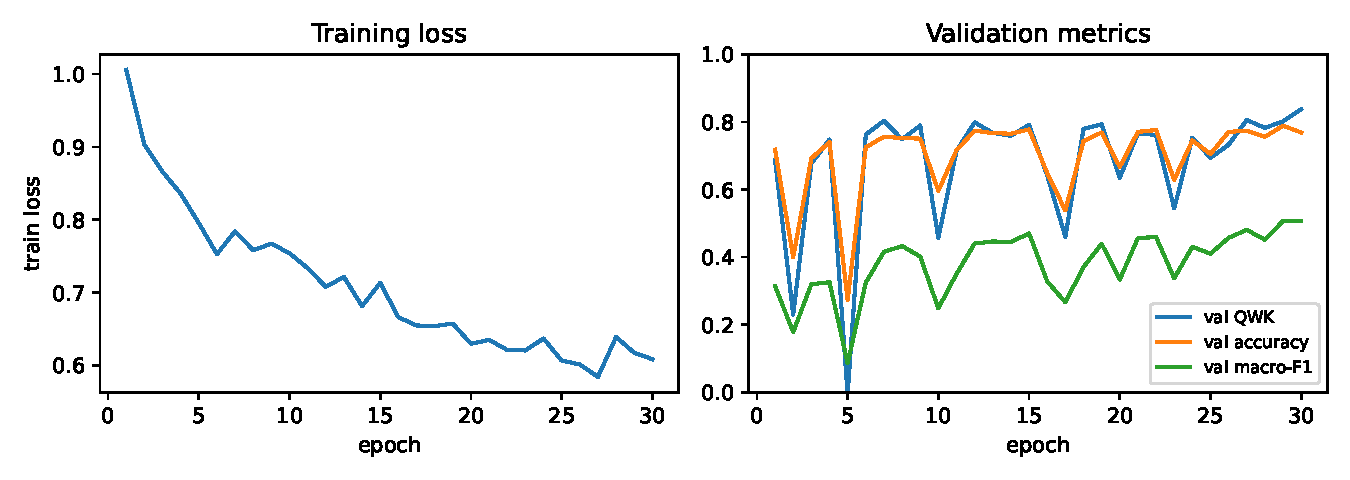
\includegraphics[width=\columnwidth]{s2_faithful_curves.pdf}
\caption{Training loss and validation metrics, strategy~2 with the paper's lr $10^{-3}$.}
\label{fig:curves}
\end{figure}

\subsection{Per-grade behaviour}
QWK and accuracy hide a severe minority-grade failure (Table~\ref{tab:perclass}, Fig.~\ref{fig:cm}).
No DR (recall 0.96) and Moderate (0.93) are learned well, but \textbf{Severe NPDR is never predicted}
(recall 0.00 in every snapshot), PDR recall is 0.30 for the single model and 0.00 for the vote, and Mild
recall is 0.23. Severe cases are split between Moderate (15/29) and PDR (13/29), and 27 of 44 PDR eyes are
called Moderate. The errors are mostly adjacent-grade, which is why QWK stays near 0.83 even though two of five
grades are essentially unrecognised; this is exactly the ``accuracy (and even QWK) can be misleading'' gap
identified in our literature review.

\begin{figure}[t]
\centering
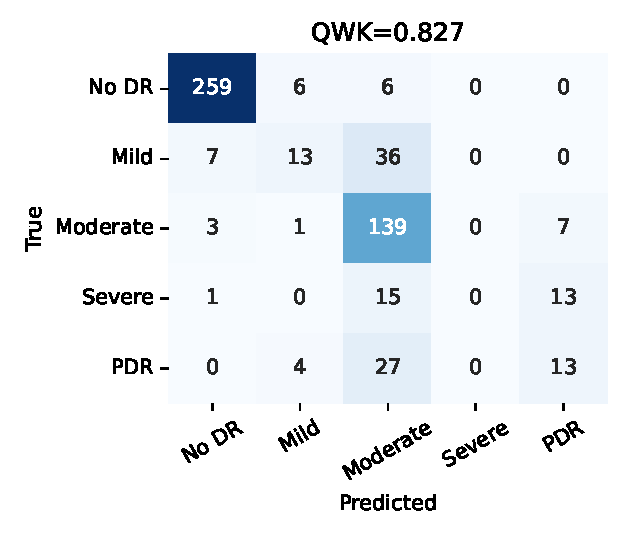
\includegraphics[width=0.78\columnwidth]{s2_faithful_best_val_cm.pdf}
\caption{Test confusion matrix of the reproduced single model (paper hyper-parameters).}
\label{fig:cm}
\end{figure}

\IfFileExists{sections/diagnostic.tex}{\subsection{Diagnostic: learning rate $10^{-4}$}
To test whether optimisation explains the gap, we repeated strategy~2 with a single change, lr
$10^{-3}\to10^{-4}$ (same split, seed, resolution, epochs and snapshots). Training became stable (no collapses;
training loss 0.27--0.32 after 20 epochs versus 0.61 at the end of the paper-setting run) and every
metric improved (Table~\ref{tab:main}): QWK \SIIlowBestQWK{} for the best-validation model (epoch 11) and
\SIIlowVoteQWK{} for the 10-snapshot vote, accuracy \SIIlowVoteAcc{}, macro-F1 \SIIlowBestMF{}.
Minority recall (mean of Severe and PDR) rose from \SIIBestMinRec{} to \SIIlowBestMinRec{}: Severe 0.00$\to$0.31
and PDR 0.30$\to$0.55 for the single model, and predictions off by two or more grades halved (48$\to$24).
With stable training the snapshots are uniformly good (test QWK 0.834--0.875), and the vote now matches the
best single model, consistent with the snapshot-ensemble assumption that members are of comparable quality.

This closes about half of the gap to 0.954 (remaining $\approx$0.07 QWK) and indicates that the paper's stated
learning rate, at least at our batch size, is the main cause of the faithful run's poor result. Severe NPDR
remains the weakest grade (single-model recall 0.31; 0.10 for the vote), and Mild is still mostly confused with
Moderate (24/56). Leakage again has no measurable effect (QWK 0.887 with and without the 29 duplicated test
images). This run is the baseline we will carry into Stage~4.
}{}

\subsection{Reproduction-gap analysis}
\label{sec:gap}
\begin{itemize}
\item \textbf{Duplicate leakage does not explain it.} Excluding the 29 test images with an identical copy in
training changes QWK from 0.827 to 0.828. The leaked images are actually predicted \emph{worse} (65.5\%
accuracy), because several copies carry conflicting grades.
\item \textbf{Optimisation (learning rate).} Full fine-tuning with Adam at $10^{-3}$, gradient clipping at 0.1
and batch size 8 is unstable (repeated collapses). The paper's own Table~3, where VGG and ResNet models predict
only class~0 under the same settings, is consistent with this. See the diagnostic run below.
\item \textbf{Resolution and schedule.} We trained at 224\,px for 30 epochs instead of 300\,px for 60; small
lesions (microaneurysms) that separate Mild from No DR and Severe from Moderate are less visible at lower
resolution.
\item \textbf{Unreported details.} Split, batch size, loss, CLAHE parameters, and whether the reported model is
the final or the best-validation one are not stated; each can move QWK by a few points on a 550-image test set.
\item \textbf{Reported numbers.} The internal inconsistencies noted in Sec.~2 (e.g.\ identical precision, recall
and QWK; macro AUC below 0.5) mean the reported 0.954 may itself not be reliable.
\end{itemize}

\subsection{Failure cases}
Fig.~\ref{fig:fail} shows the most confidently wrong test predictions. Most are PDR eyes predicted as Mild or
Moderate, including one with a large pre-retinal haemorrhage; several are dim, low-contrast or partially cropped
photographs, where neovascularisation is hard to see at 224\,px.

\begin{figure*}[t]
\centering
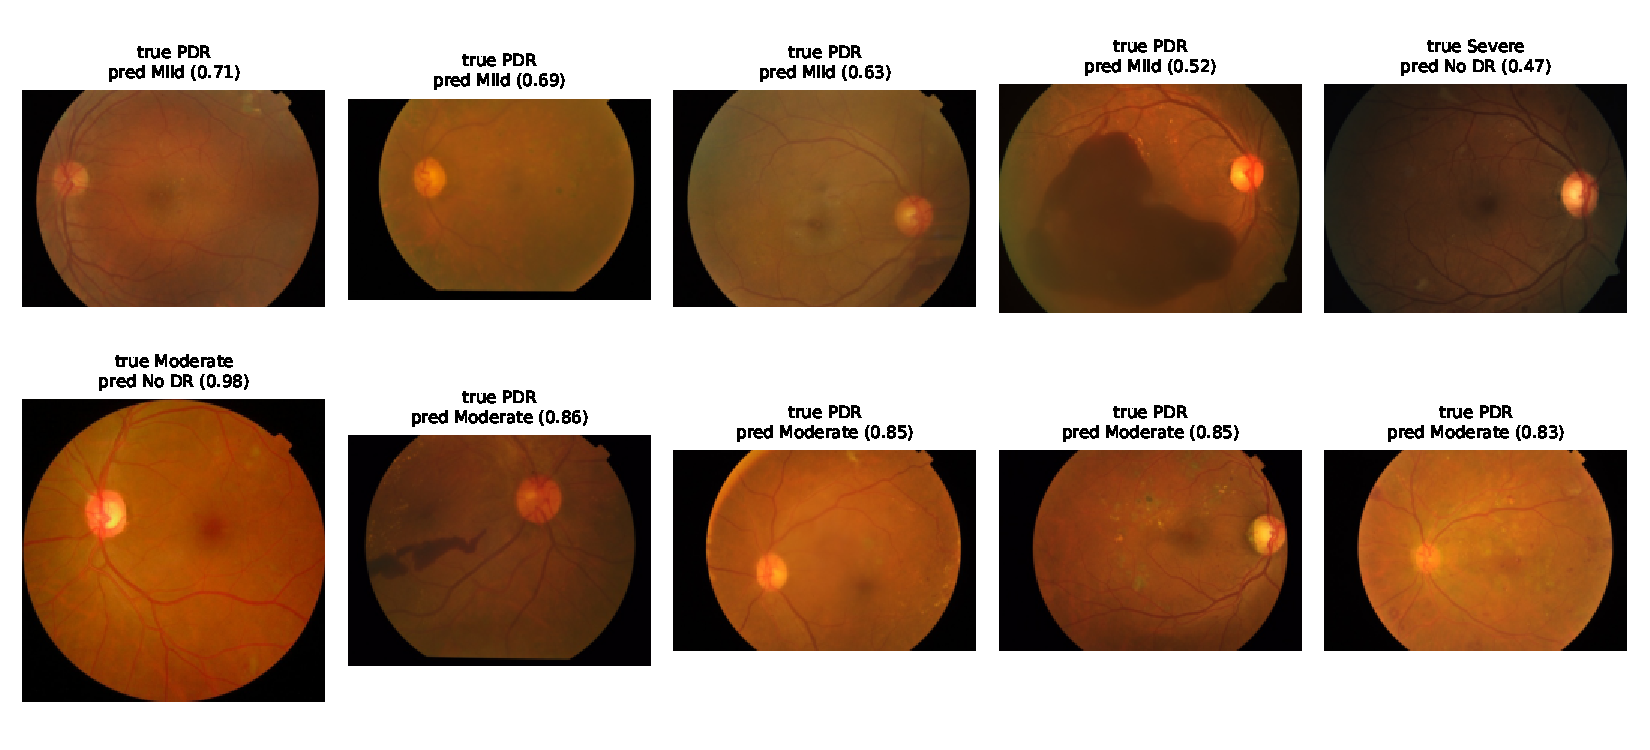
\includegraphics[width=0.9\textwidth]{s2_faithful_failures.pdf}
\caption{Ten largest-error test predictions of the reproduced single model (true grade, predicted grade, confidence).}
\label{fig:fail}
\end{figure*}

\section{Limitations}
Single dataset (APTOS~2019) and a single seed; no external validation; 224\,px / 30-epoch protocol instead of
300\,px / 60 epochs because of local hardware; the EyePACS-pretrained configuration (0.967) was not reproduced.
The 550-image test set contains only 29 Severe and 44 PDR images, so per-grade recall estimates are noisy.
This is a reproduction study; no clinical claims are made.

\section{Next Step (Stage 4 preview)}
The reproduction shows that the paper's pipeline fails on exactly the grades that matter most clinically. Our
Stage~4 hypothesis will therefore change one variable, the training loss, from cross-entropy to a
class-balanced, ordinal-aware objective, on top of the stable lr-$10^{-4}$ baseline (QWK 0.887, Severe recall
0.31), and will be stated with a predicted
direction and magnitude before any code is run.
}{}

\bibliographystyle{IEEEtran}
\bibliography{refs}
\end{document}
